\section{Machine Learning}

In traditional programming, we provide a computer with both data and a program, and it produces an output based on the instructions we've given. 
In contrast, with Machine Learning, we feed the computer data and corresponding outputs. 
The computer then trains itself by adjusting its parameters to minimize a loss function, ultimately producing a trained model that can make predictions.
\begin{figure}[H]
    \centering
    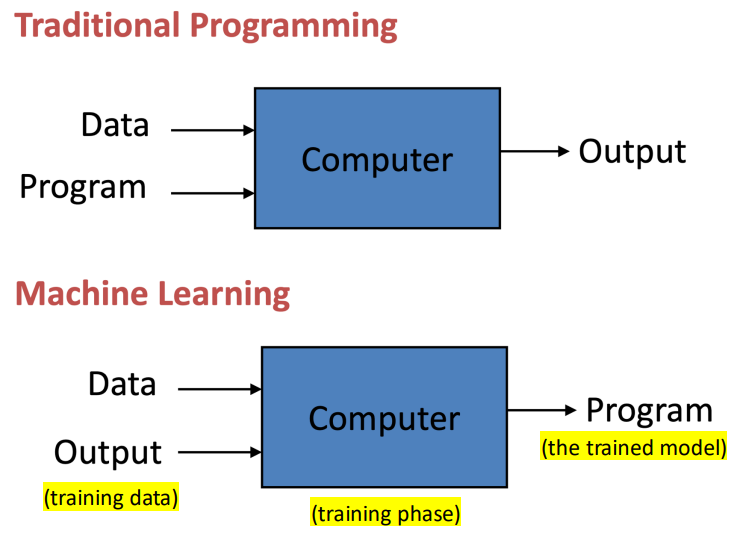
\includegraphics[width=0.4\linewidth]{images/eeai6.png}
    \caption{Traditional programming and Machine Learning}
\end{figure}
\noindent An essential aspect of Machine Learning is choosing the right model for the task. 
We aim to select a model that minimizes the error when classifying the training data. 
Models can belong to various families, such as linear or polynomial models, neural networks, and more.

\subsection{Supervised Learning}
Let's consider a simple two-dimensional problem. 
Designing a classifier requires us to identify a function that separates the labeled data points. 
Some key aspects to focus on include:
\begin{itemize}
    \item Linear or nonlinear approaches. 
    \item The number of points available or the total number of points. 
    \item The choice of technique for designing the classifier.
\end{itemize}

\paragraph*{Regression}
In nonlinear regression, given a set of noisy data points $(x_i,y_i)$, the goal is to reconstruct the underlying function. 
This is expressed as:
\[y(x,\mathbf{w})=\sum_{j=0}^{M}w_jx^j\]
\noindent To train the model, we minimize the Residual Sum of Squares with the following formula:
\[\mathcal{L}(\mathbf{w})=\dfrac{1}{2}\sum_{n=1}^N\left(y(x_n,\mathbf{w})-t_n\right)^2\]
Here, $y(x_n,\mathbf{w})$  is the model's output for the input sample $x_n$, $x_n$ represents the input data, and $t_n$ is the target value (the expected output for a given input).

\paragraph*{Training}
The training error isn't always reliable because it only measures the performance of the model on the data used for training. 
To get a better understanding of how well the model generalizes, we need to split the dataset into a training set and a test set, ensuring that the model isn't tested on the same data it was trained on.

Typically, the test error will be higher than the training error, as the model is being evaluated on unseen data. 
The amount of data we have plays a crucial role in determining the final quality of the model (more data generally leads to better results).

Additionally, we can introduce a validation set. 
This allows us to adjust the complexity of the model based on the available data, helping to avoid overfitting or underfitting the model to the training data.